\documentclass[aspectratio=169,11pt]{beamer}
\usetheme{default}
\usefonttheme{serif}
\setbeamertemplate{navigation symbols}{}
\setbeamertemplate{itemize items}[circle]

\usepackage[T1]{fontenc}
\usepackage{lmodern}
\usepackage{tikz}
\usetikzlibrary{arrows.meta,positioning}
\usepackage{pgfplots}
\pgfplotsset{compat=1.18}
\usepackage{booktabs}
\usepackage{xcolor}

\definecolor{ink}{HTML}{1F2328}
\definecolor{muted}{HTML}{6A737D}
\definecolor{faint}{HTML}{EEF0F3}
\definecolor{accent}{HTML}{1F6FEB}
\definecolor{good}{HTML}{1A7F37}
\definecolor{bad}{HTML}{CF222E}
\definecolor{warn}{HTML}{BF8700}
\definecolor{g1}{HTML}{C9D1D9}
\definecolor{g2}{HTML}{8C959F}
\definecolor{g3}{HTML}{57606A}

\setbeamercolor{normal text}{fg=ink}
\setbeamercolor{frametitle}{fg=ink}
\setbeamercolor{structure}{fg=accent}
\setbeamercolor{block title}{bg=faint,fg=ink}
\setbeamercolor{block body}{bg=faint!50,fg=ink}
\setbeamercolor{block title example}{bg=good!12,fg=ink}
\setbeamercolor{block body example}{bg=good!6,fg=ink}
\setbeamercolor{block title alerted}{bg=warn!15,fg=ink}
\setbeamercolor{block body alerted}{bg=warn!8,fg=ink}
\setbeamerfont{frametitle}{size=\Large,series=\bfseries}

\setbeamertemplate{frametitle}{%
  \vspace{0.4em}\insertframetitle\par\vspace{-0.2em}%
  {\color{g1}\rule{\textwidth}{0.4pt}}}
\setbeamertemplate{footline}{%
  \hspace{1.2em}{\color{muted}\scriptsize\insertsection}\hfill{\color{muted}\scriptsize\insertframenumber\,/\,\inserttotalframenumber}\hspace{1.2em}\vspace{0.55em}}

\newcommand{\src}[1]{\par\vfill\begin{minipage}{0.96\textwidth}\color{muted}\tiny #1\end{minipage}\vspace{-0.15em}}
\newcommand{\takeaway}[1]{\par\vfill\begin{center}\colorbox{accent!8}{\parbox{0.9\textwidth}{\centering\small #1}}\end{center}\vspace{0.2em}}
\newcommand{\sample}[2]{%
  \colorbox{#1}{\parbox{0.9\linewidth}{\footnotesize\ttfamily #2}}}

\pgfplotsset{
  deck/.style={
    ybar, bar shift=0pt, axis lines*=left, ymajorgrids, grid style={faint},
    tick label style={font=\footnotesize, color=ink},
    label style={font=\footnotesize, color=ink},
    xticklabel style={align=center, font=\footnotesize},
    nodes near coords, clip=false,
    every node near coord/.append style={font=\scriptsize, color=ink,
      /pgf/number format/fixed, /pgf/number format/precision=1},
    enlarge x limits=0.25,
  },
}

\begin{document}

%=============================================================
\begin{frame}[plain]
  \vspace{2.2em}
  \begin{center}
  {\color{muted}\small Research update \;$\cdot$\; November 2026}\\[1.1em]
  {\LARGE\bfseries Short Answer or Long Answer?}\\[0.5em]
  {\large How a small math model should answer when\\many people are waiting}\\[1.6em]
  {\normalsize Sagnik Biswas}\\[2.2em]
  {\color{muted}\footnotesize Model: Ouro-1.4B \;$\cdot$\; Problems: the MATH competition set}
  \end{center}
\end{frame}

%=============================================================
\section{Background}

\begin{frame}{The question}
  \vspace{0.4em}
  \begin{center}
  {\large When an AI model solves a math problem, should it\\[0.2em]
  \textbf{answer briefly} or \textbf{think out loud at length}?}
  \end{center}
  \vspace{0.5em}
  \begin{itemize}\setlength\itemsep{0.45em}
    \item A model writes one \textbf{token} at a time, roughly three quarters of a word.
      So a longer answer takes proportionally longer.
    \item In a real service one GPU answers many people at once (here, up to 32 questions).
      A long answer holds its place longer, and everyone behind it waits.
    \item Thinking longer might get more problems right.
  \end{itemize}
  \takeaway{We measure the trade-off: how much accuracy the long answer buys, and how much time it costs.}
\end{frame}

%-------------------------------------------------------------
\begin{frame}{The model and its two habits}
  \small
  \textbf{Ouro-1.4B} is a small model that runs each token through the same layers several times.
  The number of passes is the \textbf{depth}; we use depth 3.
  Its first token decides which of two kinds of answer it writes:
  \vspace{0.5em}
  \begin{columns}[T,onlytextwidth]
    \begin{column}{0.47\textwidth}
      \textbf{Short solution}\\[0.3em]
      \sample{accent!10}{To determine x, we start by ...}\\[0.4em]
      A compact worked solution. Starts with ``To'' 96\% of the time.
    \end{column}
    \begin{column}{0.47\textwidth}
      \textbf{Long monologue}\\[0.3em]
      \sample{g3!12}{<think> Okay, so I need to ...}\\[0.4em]
      Free-form thinking out loud. Often very long.
    \end{column}
  \end{columns}
  \vspace{0.6em}
  Left alone, the model picks the monologue for about 43\% of its answers.
  \takeaway{Because the first token decides, we can force the short habit by writing ``To'' ourselves.
  This does not switch reasoning off.}
\end{frame}

%-------------------------------------------------------------
\begin{frame}{How we score an answer}
  \vspace{0.2em}
  \begin{center}
  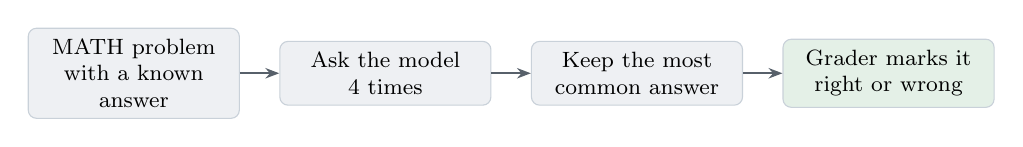
\begin{tikzpicture}[
      box/.style={draw=g1, fill=faint, rounded corners=3pt, align=center, font=\footnotesize, inner sep=4pt, text width=2.4cm},
      arr/.style={-{Stealth[length=5pt]}, thick, g3}]
    \node[box] (q) {MATH problem\\with a known answer};
    \node[box, right=0.5cm of q] (s) {Ask the model\\4 times};
    \node[box, right=0.5cm of s] (v) {Keep the most\\common answer};
    \node[box, right=0.5cm of v, fill=good!12] (g) {Grader marks it\\right or wrong};
    \draw[arr] (q) -- (s); \draw[arr] (s) -- (v); \draw[arr] (v) -- (g);
  \end{tikzpicture}
  \end{center}
  \vspace{0.3em}
  \small
  \begin{itemize}\setlength\itemsep{0.3em}
    \item \textbf{MATH} is a standard set of competition problems. \textbf{Accuracy} is the share answered correctly.
    \item Every answer has a length limit, the \textbf{cap}: 2{,}048 tokens (about 1{,}500 words) or 4{,}096.
      An answer that hits the cap before finishing gives \textbf{no answer}.
  \end{itemize}
  \vspace{0.2em}
  \begin{center}
  \begin{tabular}{@{}l r@{}}
    \toprule
    \textbf{Answers cut off by the cap} & \textbf{Share} \\
    \midrule
    Model picks its own habit, cap 2{,}048 & 27\% \\
    Model picks its own habit, cap 4{,}096 & 18\% \\
    Short solution, cap 2{,}048 & 3\% \\
    \bottomrule
  \end{tabular}
  \end{center}
\end{frame}

%-------------------------------------------------------------
\begin{frame}{Two safeguards against fooling ourselves}
  \small
  \begin{columns}[T,onlytextwidth]
    \begin{column}{0.48\textwidth}
      \begin{block}{Practice set and fresh set}
        Ideas are formed on \textbf{400 practice problems}.
        They count only if they hold up on \textbf{200 fresh problems} held back until then.
      \end{block}
    \end{column}
    \begin{column}{0.48\textwidth}
      \begin{block}{Real difference or luck?}
        Count problems where only one setup was right.
        8 to 5 is like 8 heads in 13 coin flips: luck. 36 to 11 is not.
        The \textbf{$p$-value} is how often luck gives a split that lopsided; below 0.05 counts as real.
      \end{block}
    \end{column}
  \end{columns}
  \vspace{0.8em}
  The three setups we compare. Same model, depth 3, same problems, same GPU:
  \vspace{0.2em}
  \begin{center}
  \renewcommand{\arraystretch}{1.15}
  \begin{tabular}{@{}l l r@{}}
    \toprule
    \textbf{Setup} & \textbf{How the answer starts} & \textbf{Cap} \\
    \midrule
    {\color{g3}\textbf{Model chooses}} & the model picks its own habit & 2{,}048 \\
    {\color{accent}\textbf{Short}} & we write ``To'' first & 2{,}048 \\
    {\color{good}\textbf{Longer cap}} & the model picks its own habit & 4{,}096 \\
    \bottomrule
  \end{tabular}
  \end{center}
\end{frame}

%=============================================================
\section{Experiments}

\begin{frame}{Short looked more accurate, then it wasn't}
  \small
  \begin{columns}[T,onlytextwidth]
    \begin{column}{0.5\textwidth}
      \centering\textbf{Practice set, 400 problems}\\[0.2em]
      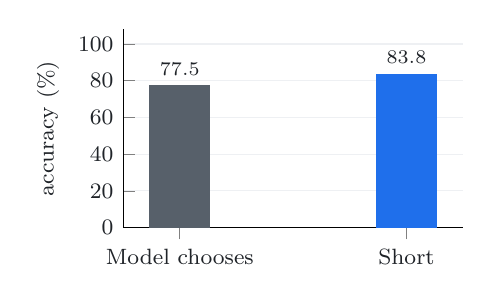
\begin{tikzpicture}
        \begin{axis}[deck, width=5.9cm, height=4.1cm, bar width=22pt,
            ymin=0, ymax=108, ylabel={accuracy (\%)},
            ytick={0,20,40,60,80,100}, xtick={0,1},
            xticklabels={{Model chooses},{Short}}]
          \addplot[fill=g3, draw=none] coordinates {(0,77.5)};
          \addplot[fill=accent, draw=none] coordinates {(1,83.8)};
        \end{axis}
      \end{tikzpicture}\\[0.2em]
      Short wins 36 to 11. $p = 0.00035$. Looks real.
    \end{column}
    \begin{column}{0.5\textwidth}
      \centering\textbf{Fresh set, 200 problems}\\[0.2em]
      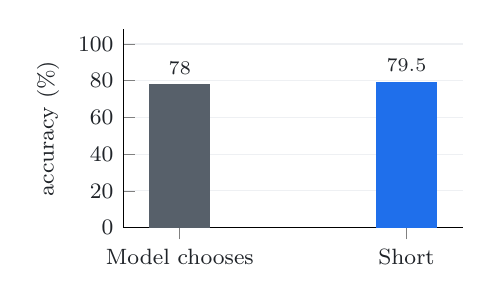
\begin{tikzpicture}
        \begin{axis}[deck, width=5.9cm, height=4.1cm, bar width=22pt,
            ymin=0, ymax=108, ylabel={accuracy (\%)},
            ytick={0,20,40,60,80,100}, xtick={0,1},
            xticklabels={{Model chooses},{Short}}]
          \addplot[fill=g3, draw=none] coordinates {(0,78.0)};
          \addplot[fill=accent, draw=none] coordinates {(1,79.5)};
        \end{axis}
      \end{tikzpicture}\\[0.2em]
      Short wins 8 to 5. $p = 0.58$. Luck.
    \end{column}
  \end{columns}
  \takeaway{We withdrew the claim that Short is more accurate.
  On practice problems, 30\% of model-chooses answers were cut off by the cap, against 2\% of Short.}
\end{frame}

%-------------------------------------------------------------
\begin{frame}{What actually helps: letting the monologue finish}
  \small
  \begin{columns}[c,onlytextwidth]
    \begin{column}{0.55\textwidth}
      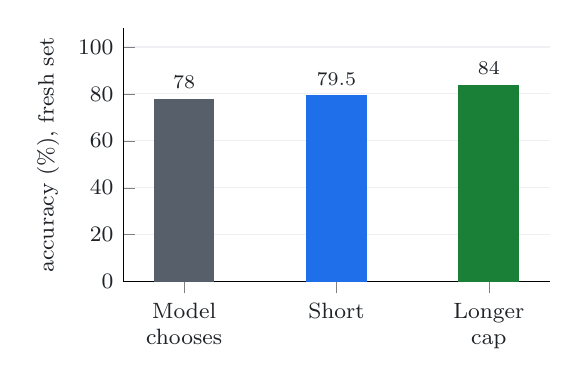
\begin{tikzpicture}
        \begin{axis}[deck, width=7.0cm, height=4.8cm, bar width=22pt,
            ymin=0, ymax=108, ylabel={accuracy (\%), fresh set}, enlarge x limits=0.2,
            ytick={0,20,40,60,80,100}, xtick={0,1,2},
            xticklabels={{Model\\chooses},{Short},{Longer\\cap}}]
          \addplot[fill=g3, draw=none] coordinates {(0,78.0)};
          \addplot[fill=accent, draw=none] coordinates {(1,79.5)};
          \addplot[fill=good, draw=none] coordinates {(2,84.0)};
        \end{axis}
      \end{tikzpicture}
    \end{column}
    \begin{column}{0.43\textwidth}
      Doubling the cap to 4{,}096 gains \textbf{6 points}: 15 problems won, 3 lost, $p = 0.0075$.\\[0.6em]
      It also beats Short by \textbf{4.5 points}: 11 won, 2 lost, $p = 0.022$.\\[0.6em]
      Both hold on fresh problems. The longer cap also gained 5 points on the practice set.
    \end{column}
  \end{columns}
\end{frame}

%-------------------------------------------------------------
\begin{frame}{The cost is time}
  \small
  \begin{columns}[c,onlytextwidth]
    \begin{column}{0.55\textwidth}
      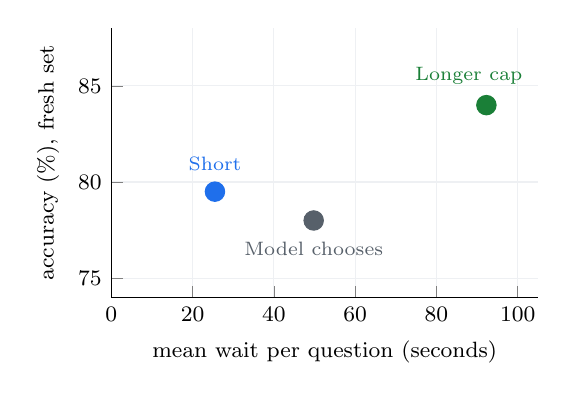
\begin{tikzpicture}
        \begin{axis}[width=7.0cm, height=5.0cm, axis lines*=left,
            xmin=0, xmax=105, ymin=74, ymax=88,
            xlabel={mean wait per question (seconds)}, ylabel={accuracy (\%), fresh set},
            grid=major, grid style={faint},
            tick label style={font=\footnotesize}, label style={font=\footnotesize}, clip=false]
          \addplot[only marks, mark=*, mark size=3.5pt, g3] coordinates {(49.8,78.0)};
          \addplot[only marks, mark=*, mark size=3.5pt, accent] coordinates {(25.5,79.5)};
          \addplot[only marks, mark=*, mark size=3.5pt, good] coordinates {(92.3,84.0)};
          \node[font=\scriptsize, anchor=north, color=g3] at (axis cs:49.8,77.4) {Model chooses};
          \node[font=\scriptsize, anchor=south, color=accent] at (axis cs:25.5,80.1) {Short};
          \node[font=\scriptsize, anchor=south, color=good] at (axis cs:88,84.6) {Longer cap};
        \end{axis}
      \end{tikzpicture}
    \end{column}
    \begin{column}{0.43\textwidth}
      \renewcommand{\arraystretch}{1.15}
      \begin{tabular}{@{}l r r@{}}
        \toprule
        & \textbf{Wait} & \textbf{Per min} \\
        \midrule
        \textcolor{accent}{Short} & 25.5 s & 20.4 \\
        \textcolor{g3}{Model chooses} & 49.8 s & 11.5 \\
        \textcolor{good}{Longer cap} & 92.3 s & 6.5 \\
        \bottomrule
      \end{tabular}\\[0.7em]
      Short is the fastest. Longer cap is the most accurate and about 3.6 times slower.
      Model chooses is slower than Short and no more accurate.
    \end{column}
  \end{columns}
  \src{Wait: seconds from when the GPU picks up a question until its last answer finishes. Per min: questions finished per minute. One timed run per setup.}
\end{frame}

%-------------------------------------------------------------
\begin{frame}{Two side checks, on the practice set}
  \small
  \begin{columns}[T,onlytextwidth]
    \begin{column}{0.48\textwidth}
      \begin{block}{Does more looping help?}
        Short answers at different depths:\\[0.4em]
        \begin{tabular}{@{}l r@{}}
          Depth 2 & 75.0\% \\
          Depth 3 & 83.8\% \\
          Depth 4 & 83.8\% \\
        \end{tabular}\\[0.4em]
        Dropping to 2 passes clearly hurts. Going to 4 changes nothing.
        So depth 3 is used everywhere.
      \end{block}
    \end{column}
    \begin{column}{0.48\textwidth}
      \begin{block}{Can the monologue rescue hard problems?}
        On 75 problems where the four short answers never reached 3-of-4 agreement:\\[0.4em]
        \begin{tabular}{@{}l r@{}}
          Two long monologues & 28.0\% \\
          The short vote alone & 30.7\% \\
        \end{tabular}\\[0.4em]
        83\% of those monologues hit the cap. On the hardest problems they run out of room too.
      \end{block}
    \end{column}
  \end{columns}
\end{frame}

%=============================================================
\section{Deadline experiment}

\begin{frame}{Experiment 4: a queue with a deadline}
  \small
  Now we act like a real service. Questions arrive over time, in alternating quiet (4 per minute)
  and busy (12 per minute) stretches. Each has a \textbf{4-minute deadline}.
  A question scores only if its answer is \textbf{right and on time}.
  \vspace{0.5em}
  \begin{center}
  \renewcommand{\arraystretch}{1.2}
  \begin{tabular}{@{}l p{8.4cm}@{}}
    \toprule
    \textbf{Rule} & \textbf{Which questions get the long answer (cap 4{,}096)} \\
    \midrule
    25\% / 50\% / 75\% long & A fixed, random-looking share of the questions \\
    Long when unsure & Start with four short answers. Add the long answer only if 3-of-4 agreement is already impossible \\
    \bottomrule
  \end{tabular}
  \end{center}
  \takeaway{This step only chooses which rule to carry into the real test.}
  \src{Practice set, 400 problems, depth 3, up to 32 at a time.}
\end{frame}

%-------------------------------------------------------------
\begin{frame}{Experiment 4 results}
  \small
  \begin{center}
  \renewcommand{\arraystretch}{1.1}
  \begin{tabular}{@{}l r r r@{}}
    \toprule
    \textbf{Rule} & \textbf{Right and on time} & \textbf{Sent long} & \textbf{Missed deadline} \\
    \midrule
    25\% long & \textbf{329} & 94 & 0 \\
    50\% long & 328 & 187 & 13 \\
    75\% long & 315 & 298 & 43 \\
    Long when unsure & \textbf{329} & 69 & 37 \\
    \bottomrule
  \end{tabular}
  \end{center}
  \vspace{0.2em}
  Sending most questions long costs answers. Two rules tie at 329 of 400 (82\%);
  the tie-break written in advance prefers fewer long answers, so \textbf{``Long when unsure'' is chosen}.
  \vspace{0.4em}
  \begin{alertblock}{Not yet known}
    Whether any mix beats always-short or always-long, whether it holds on fresh problems,
    and whether it is stable. Each rule ran once. Those runs are the next step.
  \end{alertblock}
\end{frame}

%=============================================================
\section{Summary}

\begin{frame}{Summary}
  \vspace{0.3em}
  \begin{enumerate}\setlength\itemsep{0.55em}
    \item \textbf{Short answers are the fast option.} About 26 seconds and 20 questions per minute.
    \item \textbf{They are not more accurate.} The practice-set advantage did not hold on fresh problems.
    \item \textbf{Long answers are more accurate when allowed to finish.} Doubling the cap adds 6 points (78\% to 84\%), at about 92 seconds per question.
    \item \textbf{Under a deadline, sending most questions long costs answers.} We have chosen a mixing rule. Whether it beats always-short or always-long is the next test.
  \end{enumerate}
  \src{Fresh-set results: 200 MATH problems, depth 3, one run each. Deadline results: 400 practice problems, one run each.}
\end{frame}

\end{document}
